\subsection{Architectural Description}
The software architecture is comprised of several subsystems, which have different responsibilities in the system.

\begin{figure}
	\centering
	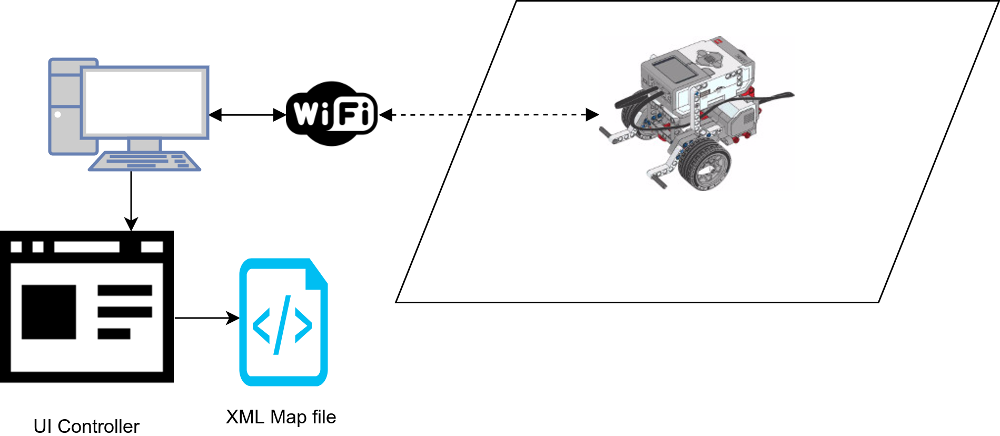
\includegraphics[width=0.9\textwidth]{Robot_system.png}	
	\caption{\label{fig:erd}This needs to be updated though}
\end{figure}	

\subsection{Component Decomposition Description}
The system has been broken down into clearly defined components, which can be tested individually. Each of these components perform a function in the entire system.

\begin{tabular}{|c|l|}
	\hline 
	\bf{Location} & \bf{Description} \\ 
	\hline 
	\hline 
	Ev3 Robot & Embedded control software \\ 
	\hline 
	PC & UI display \\ 
	\hline 
	PC & Robot Control Services \\ 
	\hline 
	PC & Robot State Logic \\ 
	\hline 
\end{tabular} 

\subsection{Detailed Components Design Description}
\subsubsection{C01 Movement Service}
\begin{itemize}
	\item Purpose: 
	\item Function: To provide a simple abstraction to move the robot.
	\item Subordinates: 
	\item Dependencies: 
	\item Interfaces: 
	\begin{itemize}
		\item 
	\end{itemize}
	\item Data: 
\end{itemize}

\subsubsection{C02 Sensors Service}

\subsubsection{C03 Robot State Machine}

\subsubsection{C04 Shared Core}

\subsubsection{C05 User Interface}

\subsubsection{C06 UI Updater}

\subsection{Architectural Alternatives}
\subsection{Design Rationale}
